%<*manuscript|acmsmall|acmsmall-submission|acmsmall-biblatex|acmlarge|acmtog|sigconf|sigconf-biblatex|authordraft|sigplan|sigchi|sigchi-a|acmsmall-conf|sigconf-i13n|acmcp>
%%
%% 
%% Commands for TeXCount
%<<TCMACROS
%TC:macro \cite [option:text,text]
%TC:macro \citep [option:text,text]
%TC:macro \citet [option:text,text]
%TC:envir table 0 1
%TC:envir table* 0 1
%TC:envir tabular [ignore] word
%TC:envir displaymath 0 word
%TC:envir math 0 word
%TC:envir comment 0 0
%TCMACROS
%% 
%% 
%% The first command in your LaTeX source must be the \documentclass
%% command.
%%
%% For submission and review of your manuscript please change the
%% command to \documentclass[manuscript, screen, review]{acmart}.
%%
%% When submitting camera ready or to TAPS, please change the command
%% to \documentclass[sigconf]{acmart} or whichever template is required
%% for your publication. 
%%
%%
%<manuscript>\documentclass[manuscript,screen,review]{acmart}
%<acmsmall|acmsmall-conf>\documentclass[acmsmall]{acmart}
%<acmsmall-biblatex>\documentclass[acmsmall,natbib=false]{acmart}
%<acmsmall-submission>\documentclass[acmsmall,screen,review]{acmart}
%<acmlarge>\documentclass[acmlarge]{acmart}
%<acmtog>\documentclass[acmtog]{acmart}
%<sigconf>\documentclass[sigconf]{acmart}
%<sigconf-biblatex>\documentclass[sigconf,natbib=false]{acmart}
%<authordraft>\documentclass[sigconf,authordraft]{acmart}
%<sigplan>\documentclass[sigplan,screen]{acmart}
%<sigchi>\documentclass[sigchi]{acmart}
%<sigchi-a>\documentclass[sigchi-a, nonacm]{acmart}
%<sigconf-i13n>\documentclass[sigconf, language=french,
%<sigconf-i13n>language=german, language=spanish, language=english]{acmart}
%<acmcp>\documentclass[acmcp]{acmart}

%%
%% \BibTeX command to typeset BibTeX logo in the docs
\AtBeginDocument{%
  \providecommand\BibTeX{{%
    Bib\TeX}}}

%% Rights management information.  This information is sent to you
%% when you complete the rights form.  These commands have SAMPLE
%% values in them; it is your responsibility as an author to replace
%% the commands and values with those provided to you when you
%% complete the rights form.
%
\setcopyright{acmcopyright}
\copyrightyear{2018}
\acmYear{2018}
\acmDOI{XXXXXXX.XXXXXXX}

%</manuscript|acmsmall|acmsmall-submission|acmsmall-biblatex|acmlarge|acmtog|sigconf|sigconf-biblatex|authordraft|sigplan|sigchi|sigchi-a|acmsmall-conf|sigconf-i13n|acmcp>
%<*manuscript|sigconf|authordraft|sigplan|sigchi|sigchi-a|acmsmall-conf|sigconf-i13n>
%% These commands are for a PROCEEDINGS abstract or paper.
\acmConference[Conference acronym 'XX]{Make sure to enter the correct
  conference title from your rights confirmation emai}{June 03--05,
  2018}{Woodstock, NY}
%%
%%  Uncomment \acmBooktitle if the title of the proceedings is different
%%  from ``Proceedings of ...''!
%%
%%\acmBooktitle{Woodstock '18: ACM Symposium on Neural Gaze Detection,
%%  June 03--05, 2018, Woodstock, NY} 
\acmPrice{15.00}
\acmISBN{978-1-4503-XXXX-X/18/06}
%</manuscript|sigconf|authordraft|sigplan|sigchi|sigchi-a|acmsmall-conf|sigconf-i13n>

%<*acmsmall|acmsmall-submission|acmsmall-biblatex|acmlarge|acmtog|acmcp>
%%
%% These commands are for a JOURNAL article.
%<acmsmall|acmsmall-submission|acmsmall-biblatex>\acmJournal{JACM}
%<acmlarge>\acmJournal{POMACS}
%<acmtog>\acmJournal{TOG}
%<acmcp>\acmJournal{JDS}
\acmVolume{37}
\acmNumber{4}
\acmArticle{111}
\acmMonth{8}
%</acmsmall|acmsmall-submission|acmsmall-biblatex|acmlarge|acmtog|acmcp>
%<*manuscript|acmsmall|acmsmall-submission|acmsmall-biblatex|acmlarge|acmtog|sigconf|sigconf-biblatex|authordraft|sigplan|sigchi|sigchi-a|acmsmall-conf|sigconf-i13n|acmcp>


%%
%% Submission ID. 
%% Use this when submitting an article to a sponsored event. You'll
%% receive a unique submission ID from the organizers
%% of the event, and this ID should be used as the parameter to this command.
%%\acmSubmissionID{123-A56-BU3}
%</manuscript|acmsmall|acmsmall-submission|acmsmall-biblatex|acmlarge|acmtog|sigconf|sigconf-biblatex|authordraft|sigplan|sigchi|sigchi-a|acmsmall-conf|sigconf-i13n|acmcp>

%<*!acmcp>
%%
%% For managing citations, it is recommended to use bibliography
%% files in BibTeX format.
%%
%% You can then either use BibTeX with the ACM-Reference-Format style,
%% or BibLaTeX with the acmnumeric or acmauthoryear sytles, that include
%% support for advanced citation of software artefact from the
%% biblatex-software package, also separately available on CTAN.
%%
%% Look at the sample-*-biblatex.tex files for templates showcasing
%% the biblatex styles.
%%
%</!acmcp>

%<*manuscript|acmsmall|acmsmall-submission|acmlarge|acmtog|sigconf|authordraft|sigplan|sigchi|sigchi-a|acmsmall-conf|sigconf-i13n>
%%
%% The majority of ACM publications use numbered citations and
%% references.  The command \citestyle{authoryear} switches to the
%% "author year" style.
%%
%% If you are preparing content for an event
%% sponsored by ACM SIGGRAPH, you must use the "author year" style of
%% citations and references.
%<!acmtog>%% Uncommenting 
%<!acmtog>%% the next command will enable that style.
%<!acmtog>%%\citestyle{acmauthoryear}
%<acmtog>\citestyle{acmauthoryear}
%</manuscript|acmsmall|acmsmall-submission|acmlarge|acmtog|sigconf|authordraft|sigplan|sigchi|sigchi-a|acmsmall-conf|sigconf-i13n>

%<*acmsmall-biblatex|sigconf-biblatex>
%%
%% The majority of ACM publications use numbered citations and
%% references, obtained by selecting the acmnumeric BibLaTeX style.
%% The acmauthoryear BibLaTeX style switches to the "author year" style.
%%
%% If you are preparing content for an event
%% sponsored by ACM SIGGRAPH, you must use the acmauthoryear style of
%% citations and references.
%%
%% Bibliography style
\RequirePackage[
  datamodel=acmdatamodel,
%<!acmsmall-biblatex>  style=acmnumeric,
%<acmsmall-biblatex>  style=acmauthoryear,
  ]{biblatex}

%% Declare bibliography sources (one \addbibresource command per source)
\addbibresource{software.bib}
\addbibresource{sample-base.bib}
%</acmsmall-biblatex|sigconf-biblatex>
%<*manuscript|acmsmall|acmsmall-submission|acmsmall-biblatex|acmlarge|acmtog|sigconf|sigconf-biblatex|authordraft|sigplan|sigchi|sigchi-a|acmsmall-conf|sigconf-i13n|acmcp>

%%
%% end of the preamble, start of the body of the document source.
\begin{document}

%%
%% The "title" command has an optional parameter,
%% allowing the author to define a "short title" to be used in page headers.
\title{The Name of the Title Is Hope}
%<sigconf-i13n>\translatedtitle{french}{Le nom du titre est l'espoir}
%<sigconf-i13n>\translatedtitle{german}{Der Name des Titels ist 'Hoffnung'}
%<sigconf-i13n>\translatedtitle{spanish}{El nombre del título es esperanza}

%%
%% The "author" command and its associated commands are used to define
%% the authors and their affiliations.
%% Of note is the shared affiliation of the first two authors, and the
%% "authornote" and "authornotemark" commands 
%% used to denote shared contribution to the research.
\author{Ben Trovato}
%<!acmcp>\authornote{Both authors contributed equally to this research.}
\email{trovato@corporation.com}
\orcid{1234-5678-9012}
\author{G.K.M. Tobin}
%<!acmcp>\authornotemark[1]
\email{webmaster@marysville-ohio.com}
\affiliation{%
  \institution{Institute for Clarity in Documentation}
  \streetaddress{P.O. Box 1212}
  \city{Dublin}
  \state{Ohio}
  \country{USA}
  \postcode{43017-6221}
}

\author{Lars Th{\o}rv{\"a}ld}
\affiliation{%
  \institution{The Th{\o}rv{\"a}ld Group}
  \streetaddress{1 Th{\o}rv{\"a}ld Circle}
  \city{Hekla}
  \country{Iceland}}
\email{larst@affiliation.org}

\author{Valerie B\'eranger}
\affiliation{%
  \institution{Inria Paris-Rocquencourt}
  \city{Rocquencourt}
  \country{France}
}

\author{Aparna Patel}
\affiliation{%
 \institution{Rajiv Gandhi University}
 \streetaddress{Rono-Hills}
 \city{Doimukh}
 \state{Arunachal Pradesh}
 \country{India}}
 
\author{Huifen Chan}
\affiliation{%
  \institution{Tsinghua University}
  \streetaddress{30 Shuangqing Rd}
  \city{Haidian Qu}
  \state{Beijing Shi}
  \country{China}}

\author{Charles Palmer}
\affiliation{%
  \institution{Palmer Research Laboratories}
  \streetaddress{8600 Datapoint Drive}
  \city{San Antonio}
  \state{Texas}
  \country{USA}
  \postcode{78229}}
\email{cpalmer@prl.com}

\author{John Smith}
\affiliation{%
  \institution{The Th{\o}rv{\"a}ld Group}
  \streetaddress{1 Th{\o}rv{\"a}ld Circle}
  \city{Hekla}
  \country{Iceland}}
\email{jsmith@affiliation.org}

\author{Julius P. Kumquat}
\affiliation{%
  \institution{The Kumquat Consortium}
  \city{New York}
  \country{USA}}
\email{jpkumquat@consortium.net}

%%
%% By default, the full list of authors will be used in the page
%% headers. Often, this list is too long, and will overlap 
%% other information printed in the page headers. This command allows
%% the author to define a more concise list 
%% of authors' names for this purpose.
\renewcommand{\shortauthors}{Trovato et al.}
%</manuscript|acmsmall|acmsmall-submission|acmsmall-biblatex|acmlarge|acmtog|sigconf|sigconf-biblatex|authordraft|sigplan|sigchi|sigchi-a|acmsmall-conf|sigconf-i13n|acmcp>
%<*acmcp>
%%
%% Article type: Research, Review, Discussion, Invited or position
\acmArticleType{Review}
%%
%% Links to code and data
\acmCodeLink{https://github.com/borisveytsman/acmart}
\acmDataLink{htps://zenodo.org/link}
%%
%%
%% Sometimes the addresses are too long to fit on the page.  In this
%% case uncomment the lines below and fill them accodingly.
%%
%% \authorsaddresses{Corresponding author: Ben Trovato,
%% \href{mailto:trovato@corporation.com}{trovato@corporation.com};
%% Institute for Clarity in Documentation, P.O. Box 1212, Dublin,
%% Ohio, USA, 43017-6221} 
%%
%</acmcp>
%<*manuscript|acmsmall|acmsmall-submission|acmsmall-biblatex|acmlarge|acmtog|sigconf|sigconf-biblatex|authordraft|sigplan|sigchi|sigchi-a|acmsmall-conf|sigconf-i13n>

%%
%% The abstract is a short summary of the work to be presented in the
%% article. 
\begin{abstract}
  A clear and well-documented \LaTeX\ document is presented as an
  article formatted for publication by ACM in a conference proceedings
  or journal publication. Based on the ``acmart'' document class, this
  article presents and explains many of the common variations, as well
  as many of the formatting elements an author may use in the
  preparation of the documentation of their work.
\end{abstract}
%</manuscript|acmsmall|acmsmall-submission|acmsmall-biblatex|acmlarge|acmtog|sigconf|sigconf-biblatex|authordraft|sigplan|sigchi|sigchi-a|acmsmall-conf|sigconf-i13n>
%<*sigconf-i13n>

\begin{translatedabstract}{french}
  Un document \LaTeX\ clair et bien documenté est présenté comme un
  article formaté pour publication par ACM dans les actes d'une
  conférence ou parution dans une revue. Basé sur la classe de
  document ``acmart'', ce l'article présente et explique de nombreuses
  variations courantes, ainsi que autant d'éléments de mise en forme
  qu'un auteur peut utiliser dans le préparation de la documentation
  de leur travail.
\end{translatedabstract}

\begin{translatedabstract}{german}
  Es wird ein übersichtliches und gut dokumentiertes \LaTeX\-Dokument präsentiert,
  welches für die Veröffentlichung durch ACM in einem Tagungsband oder
  als Zeitschriftenpublikation formatiert wurde.
  Basierend auf der Dokumentenklasse ``acmart'' präsentiert und erklärt dieser Artikel
  viele der Formatierungselemente sowie auch viele der gängigen Variationen,
  die ein Autor bei der Beschreibung seiner Arbeit verwenden darf.
\end{translatedabstract}

\begin{translatedabstract}{spanish}
  Un documento \LaTeX\ claro y bien documentado se presenta como un
  artículo formateado para su publicación por ACM en las actas de una
  conferencia o publicación de una revista. Basado en la clase de
  documento ``acmart'', este artículo presenta y explica muchas de las
  variaciones comunes, así como tantos de los elementos de formato que
  un autor puede usar en el preparación de la documentación de su
  trabajo.
 \end{translatedabstract}
%</sigconf-i13n>
%<*manuscript|acmsmall|acmsmall-submission|acmsmall-biblatex|acmlarge|acmtog|sigconf|sigconf-biblatex|authordraft|sigplan|sigchi|sigchi-a|acmsmall-conf|sigconf-i13n>

%%
%% The code below is generated by the tool at http://dl.acm.org/ccs.cfm.
%% Please copy and paste the code instead of the example below.
%%
\begin{CCSXML}
<ccs2012>
 <concept>
  <concept_id>10010520.10010553.10010562</concept_id>
  <concept_desc>Computer systems organization~Embedded systems</concept_desc>
  <concept_significance>500</concept_significance>
 </concept>
 <concept>
  <concept_id>10010520.10010575.10010755</concept_id>
  <concept_desc>Computer systems organization~Redundancy</concept_desc>
  <concept_significance>300</concept_significance>
 </concept>
 <concept>
  <concept_id>10010520.10010553.10010554</concept_id>
  <concept_desc>Computer systems organization~Robotics</concept_desc>
  <concept_significance>100</concept_significance>
 </concept>
 <concept>
  <concept_id>10003033.10003083.10003095</concept_id>
  <concept_desc>Networks~Network reliability</concept_desc>
  <concept_significance>100</concept_significance>
 </concept>
</ccs2012>
\end{CCSXML}

\ccsdesc[500]{Computer systems organization~Embedded systems}
\ccsdesc[300]{Computer systems organization~Redundancy}
\ccsdesc{Computer systems organization~Robotics}
\ccsdesc[100]{Networks~Network reliability}

%</manuscript|acmsmall|acmsmall-submission|acmsmall-biblatex|acmlarge|acmtog|sigconf|sigconf-biblatex|authordraft|sigplan|sigchi|sigchi-a|acmsmall-conf|sigconf-i13n>
%<*manuscript|acmsmall|acmsmall-submission|acmsmall-biblatex|acmlarge|acmtog|sigconf|sigconf-biblatex|authordraft|sigplan|sigchi|sigchi-a|acmsmall-conf|sigconf-i13n|acmcp>
%%
%% Keywords. The author(s) should pick words that accurately describe
%% the work being presented. Separate the keywords with commas.
\keywords{datasets, neural networks, gaze detection, text tagging}
%<sigconf-i13n>\translatedkeywords{french}{ensembles de données,
%<sigconf-i13n> réseaux de neurones,
%<sigconf-i13n>  détection du regard, marquage de texte}
%<sigconf-i13n>  \translatedkeywords{german}{Datensammlungen,
%<sigconf-i13n> neuronale Netze, Blickerkennung, Textklassifizierung}
%<sigconf-i13n> \translatedkeywords{spanish}{conjuntos de datos,
%<sigconf-i13n> redes neuronales, detección de mirada, etiquetado de texto} 
%</manuscript|acmsmall|acmsmall-submission|acmsmall-biblatex|acmlarge|acmtog|sigconf|sigconf-biblatex|authordraft|sigplan|sigchi|sigchi-a|acmsmall-conf|sigconf-i13n|acmcp>
%<*sigconf|authordraft|sigplan|acmsmall-conf|sigconf-i13n>
%% A "teaser" image appears between the author and affiliation
%% information and the body of the document, and typically spans the
%% page.
\begin{teaserfigure}
  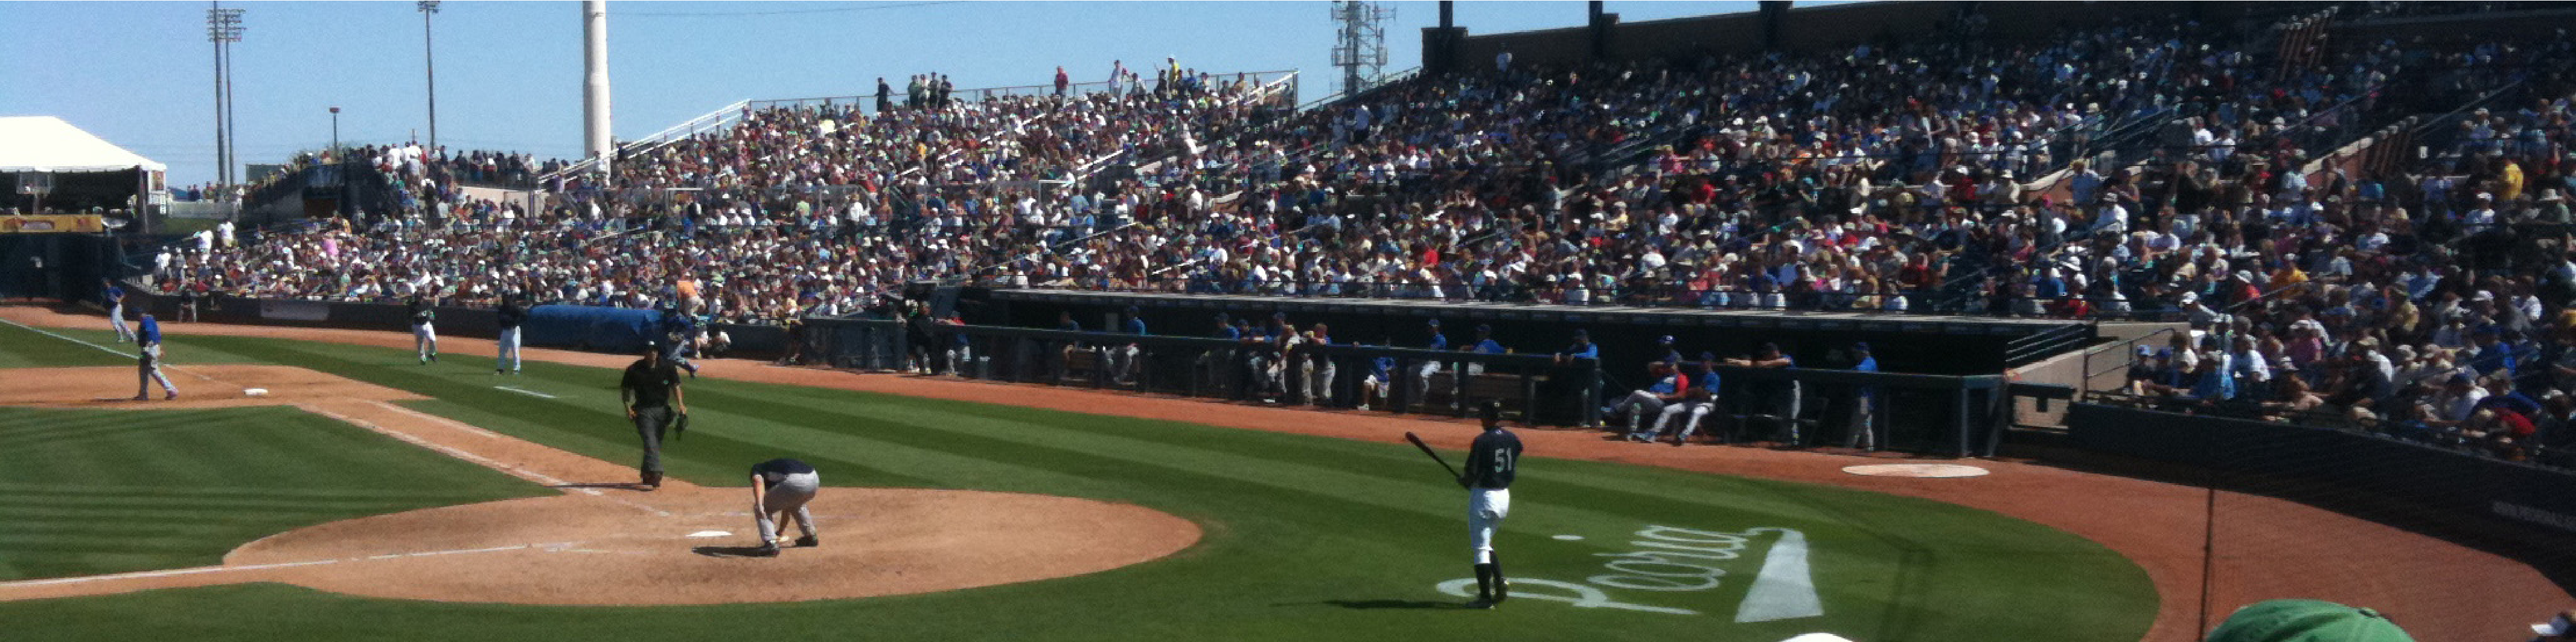
\includegraphics[width=\textwidth]{sampleteaser}
  \caption{Seattle Mariners at Spring Training, 2010.}
  \Description{Enjoying the baseball game from the third-base
  seats. Ichiro Suzuki preparing to bat.} 
  \label{fig:teaser}
\end{teaserfigure}
%</sigconf|authordraft|sigplan|acmsmall-conf|sigconf-i13n>
%<*manuscript|acmsmall|acmsmall-submission|acmsmall-biblatex|acmlarge|acmtog|sigconf|sigconf-biblatex|authordraft|sigplan|sigchi|sigchi-a|acmsmall-conf|sigconf-i13n>

\received{20 February 2007}
\received[revised]{12 March 2009}
\received[accepted]{5 June 2009}

%%
%% This command processes the author and affiliation and title
%% information and builds the first part of the formatted document.
\maketitle

\section{Introduction}
ACM's consolidated article template, introduced in 2017, provides a
consistent \LaTeX\ style for use across ACM publications, and
incorporates accessibility and metadata-extraction functionality
necessary for future Digital Library endeavors. Numerous ACM and
SIG-specific \LaTeX\ templates have been examined, and their unique
features incorporated into this single new template.

If you are new to publishing with ACM, this document is a valuable
guide to the process of preparing your work for publication. If you
have published with ACM before, this document provides insight and
instruction into more recent changes to the article template.

The ``\verb|acmart|'' document class can be used to prepare articles
for any ACM publication --- conference or journal, and for any stage
of publication, from review to final ``camera-ready'' copy, to the
author's own version, with {\itshape very} few changes to the source.

\section{Template Overview}
As noted in the introduction, the ``\verb|acmart|'' document class can
be used to prepare many different kinds of documentation --- a
double-blind initial submission of a full-length technical paper, a
two-page SIGGRAPH Emerging Technologies abstract, a ``camera-ready''
journal article, a SIGCHI Extended Abstract, and more --- all by
selecting the appropriate {\itshape template style} and {\itshape
  template parameters}.

This document will explain the major features of the document
class. For further information, the {\itshape \LaTeX\ User's Guide} is
available from
\url{https://www.acm.org/publications/proceedings-template}.

\subsection{Template Styles}

The primary parameter given to the ``\verb|acmart|'' document class is
the {\itshape template style} which corresponds to the kind of publication
or SIG publishing the work. This parameter is enclosed in square
brackets and is a part of the {\verb|documentclass|} command:
\begin{verbatim}
  \documentclass[STYLE]{acmart}
\end{verbatim}

Journals use one of three template styles. All but three ACM journals
use the {\verb|acmsmall|} template style:
\begin{itemize}
\item {\texttt{acmsmall}}: The default journal template style.
\item {\texttt{acmlarge}}: Used by JOCCH and TAP.
\item {\texttt{acmtog}}: Used by TOG.
\end{itemize}

The majority of conference proceedings documentation will use the {\verb|acmconf|} template style.
\begin{itemize}
\item {\texttt{acmconf}}: The default proceedings template style.
\item{\texttt{sigchi}}: Used for SIGCHI conference articles.
\item{\texttt{sigplan}}: Used for SIGPLAN conference articles.
\end{itemize}

\subsection{Template Parameters}

In addition to specifying the {\itshape template style} to be used in
formatting your work, there are a number of {\itshape template parameters}
which modify some part of the applied template style. A complete list
of these parameters can be found in the {\itshape \LaTeX\ User's Guide.}

Frequently-used parameters, or combinations of parameters, include:
\begin{itemize}
\item {\texttt{anonymous,review}}: Suitable for a ``double-blind''
  conference submission. Anonymizes the work and includes line
  numbers. Use with the \texttt{\acmSubmissionID} command to print the
  submission's unique ID on each page of the work.
\item{\texttt{authorversion}}: Produces a version of the work suitable
  for posting by the author.
\item{\texttt{screen}}: Produces colored hyperlinks.
\end{itemize}

This document uses the following string as the first command in the
source file:
\begin{verbatim}
%<manuscript>\documentclass[manuscript,screen,review]{acmart}
%<acmsmall|acmsmall-conf>\documentclass[acmsmall]{acmart}
%<acmsmall-submission>\documentclass[acmsmall,screen,review]{acmart}
%<acmlarge>\documentclass[acmlarge]{acmart}
%<acmtog>\documentclass[acmtog]{acmart}
%<sigconf>\documentclass[sigconf]{acmart}
%<authordraft>\documentclass[sigconf,authordraft]{acmart}
%<sigplan>\documentclass[sigplan,screen]{acmart}
%<sigchi>\documentclass[sigchi]{acmart}
%<sigchi-a>\documentclass[sigchi-a]{acmart}
%<sigconf-i13n>\documentclass[sigconf, language=french,
%<sigconf-i13n>language=german, language=spanish, language=english]{acmart}
\end{verbatim}


\section{Modifications}

Modifying the template --- including but not limited to: adjusting
margins, typeface sizes, line spacing, paragraph and list definitions,
and the use of the \verb|\vspace| command to manually adjust the
vertical spacing between elements of your work --- is not allowed.

{\bfseries Your document will be returned to you for revision if
  modifications are discovered.}

\section{Typefaces}

The ``\verb|acmart|'' document class requires the use of the
``Libertine'' typeface family. Your \TeX\ installation should include
this set of packages. Please do not substitute other typefaces. The
``\verb|lmodern|'' and ``\verb|ltimes|'' packages should not be used,
as they will override the built-in typeface families.

\section{Title Information}

The title of your work should use capital letters appropriately -
\url{https://capitalizemytitle.com/} has useful rules for
capitalization. Use the {\verb|title|} command to define the title of
your work. If your work has a subtitle, define it with the
{\verb|subtitle|} command.  Do not insert line breaks in your title.

If your title is lengthy, you must define a short version to be used
in the page headers, to prevent overlapping text. The \verb|title|
command has a ``short title'' parameter:
\begin{verbatim}
  \title[short title]{full title}
\end{verbatim}

\section{Authors and Affiliations}

Each author must be defined separately for accurate metadata
identification.  As an exception, multiple authors may share one
affiliation. Authors' names should not be abbreviated; use full first
names wherever possible. Include authors' e-mail addresses whenever
possible.

Grouping authors' names or e-mail addresses, or providing an ``e-mail
alias,'' as shown below, is not acceptable:
\begin{verbatim}
  \author{Brooke Aster, David Mehldau}
  \email{dave,judy,steve@university.edu}
  \email{firstname.lastname@phillips.org}
\end{verbatim}

The \verb|authornote| and \verb|authornotemark| commands allow a note
to apply to multiple authors --- for example, if the first two authors
of an article contributed equally to the work.

If your author list is lengthy, you must define a shortened version of
the list of authors to be used in the page headers, to prevent
overlapping text. The following command should be placed just after
the last \verb|\author{}| definition:
\begin{verbatim}
  \renewcommand{\shortauthors}{McCartney, et al.}
\end{verbatim}
Omitting this command will force the use of a concatenated list of all
of the authors' names, which may result in overlapping text in the
page headers.

The article template's documentation, available at
\url{https://www.acm.org/publications/proceedings-template}, has a
complete explanation of these commands and tips for their effective
use.

Note that authors' addresses are mandatory for journal articles.

\section{Rights Information}

Authors of any work published by ACM will need to complete a rights
form. Depending on the kind of work, and the rights management choice
made by the author, this may be copyright transfer, permission,
license, or an OA (open access) agreement.

Regardless of the rights management choice, the author will receive a
copy of the completed rights form once it has been submitted. This
form contains \LaTeX\ commands that must be copied into the source
document. When the document source is compiled, these commands and
their parameters add formatted text to several areas of the final
document:
\begin{itemize}
\item the ``ACM Reference Format'' text on the first page.
\item the ``rights management'' text on the first page.
\item the conference information in the page header(s).
\end{itemize}

Rights information is unique to the work; if you are preparing several
works for an event, make sure to use the correct set of commands with
each of the works.

The ACM Reference Format text is required for all articles over one
page in length, and is optional for one-page articles (abstracts).

\section{CCS Concepts and User-Defined Keywords}

Two elements of the ``acmart'' document class provide powerful
taxonomic tools for you to help readers find your work in an online
search.

The ACM Computing Classification System ---
\url{https://www.acm.org/publications/class-2012} --- is a set of
classifiers and concepts that describe the computing
discipline. Authors can select entries from this classification
system, via \url{https://dl.acm.org/ccs/ccs.cfm}, and generate the
commands to be included in the \LaTeX\ source.

User-defined keywords are a comma-separated list of words and phrases
of the authors' choosing, providing a more flexible way of describing
the research being presented.

CCS concepts and user-defined keywords are required for for all
articles over two pages in length, and are optional for one- and
two-page articles (or abstracts).

\section{Sectioning Commands}

Your work should use standard \LaTeX\ sectioning commands:
\verb|section|, \verb|subsection|, \verb|subsubsection|, and
\verb|paragraph|. They should be numbered; do not remove the numbering
from the commands.

Simulating a sectioning command by setting the first word or words of
a paragraph in boldface or italicized text is {\bfseries not allowed.}

\section{Tables}

The ``\verb|acmart|'' document class includes the ``\verb|booktabs|''
package --- \url{https://ctan.org/pkg/booktabs} --- for preparing
high-quality tables.

Table captions are placed {\itshape above} the table.

Because tables cannot be split across pages, the best placement for
them is typically the top of the page nearest their initial cite.  To
ensure this proper ``floating'' placement of tables, use the
environment \textbf{table} to enclose the table's contents and the
table caption.  The contents of the table itself must go in the
\textbf{tabular} environment, to be aligned properly in rows and
columns, with the desired horizontal and vertical rules.  Again,
detailed instructions on \textbf{tabular} material are found in the
\textit{\LaTeX\ User's Guide}.

Immediately following this sentence is the point at which
Table~\ref{tab:freq} is included in the input file; compare the
placement of the table here with the table in the printed output of
this document.

%<!sigchi-a>\begin{table}
%<sigchi-a>\begin{margintable}
  \caption{Frequency of Special Characters}
  \label{tab:freq}
  \begin{tabular}{ccl}
    \toprule
    Non-English or Math&Frequency&Comments\\
    \midrule
    \O & 1 in 1,000& For Swedish names\\
    $\pi$ & 1 in 5& Common in math\\
    \$ & 4 in 5 & Used in business\\
    $\Psi^2_1$ & 1 in 40,000& Unexplained usage\\
  \bottomrule
\end{tabular}
%<!sigchi-a>\end{table}
%<sigchi-a>\end{margintable}

To set a wider table, which takes up the whole width of the page's
live area, use the environment \textbf{table*} to enclose the table's
contents and the table caption.  As with a single-column table, this
wide table will ``float'' to a location deemed more
desirable. Immediately following this sentence is the point at which
Table~\ref{tab:commands} is included in the input file; again, it is
instructive to compare the placement of the table here with the table
in the printed output of this document.

\begin{table*}
  \caption{Some Typical Commands}
  \label{tab:commands}
  \begin{tabular}{ccl}
    \toprule
    Command &A Number & Comments\\
    \midrule
    \texttt{{\char'134}author} & 100& Author \\
    \texttt{{\char'134}table}& 300 & For tables\\
    \texttt{{\char'134}table*}& 400& For wider tables\\
    \bottomrule
  \end{tabular}
\end{table*}

Always use midrule to separate table header rows from data rows, and
use it only for this purpose. This enables assistive technologies to
recognise table headers and support their users in navigating tables
more easily.


\section{Math Equations}
You may want to display math equations in three distinct styles:
inline, numbered or non-numbered display.  Each of the three are
discussed in the next sections.

\subsection{Inline (In-text) Equations}
A formula that appears in the running text is called an inline or
in-text formula.  It is produced by the \textbf{math} environment,
which can be invoked with the usual
\texttt{{\char'134}begin\,\ldots{\char'134}end} construction or with
the short form \texttt{\$\,\ldots\$}. You can use any of the symbols
and structures, from $\alpha$ to $\omega$, available in
\LaTeX~\cite{Lamport:LaTeX}; this section will simply show a few
examples of in-text equations in context. Notice how this equation:
\begin{math}
  \lim_{n\rightarrow \infty}x=0
\end{math},
set here in in-line math style, looks slightly different when
set in display style.  (See next section).

\subsection{Display Equations}
A numbered display equation---one set off by vertical space from the
text and centered horizontally---is produced by the \textbf{equation}
environment. An unnumbered display equation is produced by the
\textbf{displaymath} environment.

Again, in either environment, you can use any of the symbols and
structures available in \LaTeX\@; this section will just give a couple
of examples of display equations in context.  First, consider the
equation, shown as an inline equation above:
\begin{equation}
  \lim_{n\rightarrow \infty}x=0
\end{equation}
Notice how it is formatted somewhat differently in
the \textbf{displaymath}
environment.  Now, we'll enter an unnumbered equation:
\begin{displaymath}
  \sum_{i=0}^{\infty} x + 1
\end{displaymath}
and follow it with another numbered equation:
\begin{equation}
  \sum_{i=0}^{\infty}x_i=\int_{0}^{\pi+2} f
\end{equation}
just to demonstrate \LaTeX's able handling of numbering.

\section{Figures}

The ``\verb|figure|'' environment should be used for figures. One or
more images can be placed within a figure. If your figure contains
third-party material, you must clearly identify it as such, as shown
in the example below.
%<!sigchi-a>\begin{figure}[h]
%<sigchi-a>\begin{marginfigure}
  \centering
  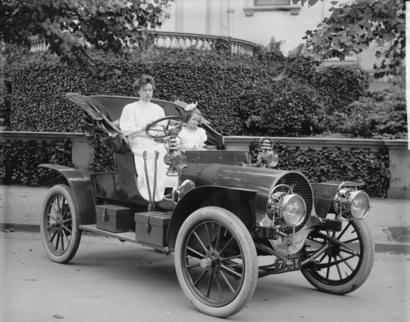
\includegraphics[width=\linewidth]{sample-franklin}
  \caption{1907 Franklin Model D roadster. Photograph by Harris \&
    Ewing, Inc. [Public domain], via Wikimedia
    Commons. (\url{https://goo.gl/VLCRBB}).}
  \Description{A woman and a girl in white dresses sit in an open car.}
%<!sigchi-a>\end{figure}
%<sigchi-a>\end{marginfigure}

Your figures should contain a caption which describes the figure to
the reader.

Figure captions are placed {\itshape below} the figure.

Every figure should also have a figure description unless it is purely
decorative. These descriptions convey what’s in the image to someone
who cannot see it. They are also used by search engine crawlers for
indexing images, and when images cannot be loaded.

A figure description must be unformatted plain text less than 2000
characters long (including spaces).  {\bfseries Figure descriptions
  should not repeat the figure caption – their purpose is to capture
  important information that is not already provided in the caption or
  the main text of the paper.} For figures that convey important and
complex new information, a short text description may not be
adequate. More complex alternative descriptions can be placed in an
appendix and referenced in a short figure description. For example,
provide a data table capturing the information in a bar chart, or a
structured list representing a graph.  For additional information
regarding how best to write figure descriptions and why doing this is
so important, please see
\url{https://www.acm.org/publications/taps/describing-figures/}.


\subsection{The ``Teaser Figure''}

A ``teaser figure'' is an image, or set of images in one figure, that
are placed after all author and affiliation information, and before
the body of the article, spanning the page. If you wish to have such a
figure in your article, place the command immediately before the
\verb|\maketitle| command:
\begin{verbatim}
  \begin{teaserfigure}
    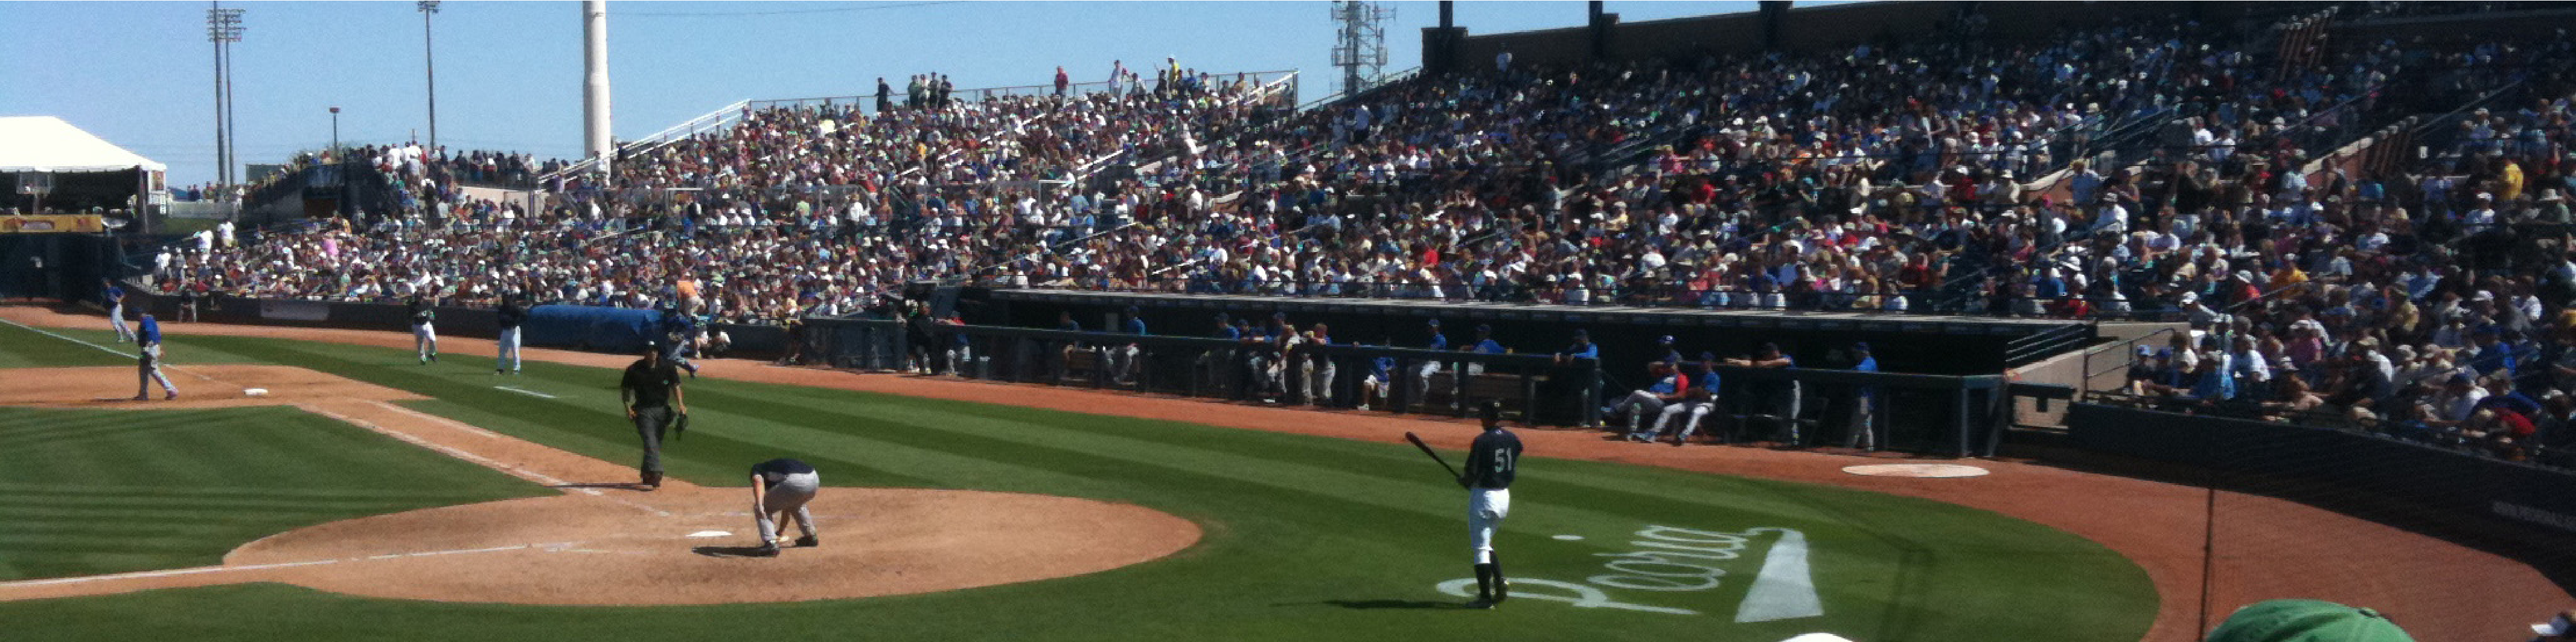
\includegraphics[width=\textwidth]{sampleteaser}
    \caption{figure caption}
    \Description{figure description}
  \end{teaserfigure}
\end{verbatim}

\section{Citations and Bibliographies}

The use of \BibTeX\ for the preparation and formatting of one's
references is strongly recommended. Authors' names should be complete
--- use full first names (``Donald E. Knuth'') not initials
(``D. E. Knuth'') --- and the salient identifying features of a
reference should be included: title, year, volume, number, pages,
article DOI, etc.

%<*!(acmsmall-biblatex|sigconf-biblatex)>
The bibliography is included in your source document with these two
commands, placed just before the \verb|\end{document}| command:
\begin{verbatim}
  \bibliographystyle{ACM-Reference-Format}
  \bibliography{bibfile}
\end{verbatim}
where ``\verb|bibfile|'' is the name, without the ``\verb|.bib|''
suffix, of the \BibTeX\ file.

Citations and references are numbered by default. A small number of
ACM publications have citations and references formatted in the
``author year'' style; for these exceptions, please include this
command in the {\bfseries preamble} (before the command
``\verb|\begin{document}|'') of your \LaTeX\ source:
\begin{verbatim}
  \citestyle{acmauthoryear}
\end{verbatim}
%</!(acmsmall-biblatex|sigconf-biblatex)>

%<*acmsmall-biblatex|sigconf-biblatex>
Using the BibLaTeX system, the bibliography is included in your source
document with the following command, placed just before the \verb|\end{document}| command:
\begin{verbatim}
  \printbibliography
\end{verbatim}

The command \verb|\addbibresource{bibfile}| declares the \BibTeX\ file to use
in the {\bfseries preamble} (before the command
``\verb|\begin{document}|'') of your \LaTeX\ source
where ``\verb|bibfile|'' is the name, \emph{with} the ``\verb|.bib|'' suffix.
Notice that \verb|\addbibresource| takes only one argument: to declare multiple files,
use multiple instances of the command.

Citations and references are numbered by default. A small number of
ACM publications have citations and references formatted in the
``author year'' style; for these exceptions, please pass the option \verb|style=acmauthoryear|
to the \verb|biblatex| package loaded in the {\bfseries preamble} (before the command
``\verb|\begin{document}|'') of your \LaTeX\ source.

%</acmsmall-biblatex|sigconf-biblatex>



  Some examples.  A paginated journal article \cite{Abril07}, an
  enumerated journal article \cite{Cohen07}, a reference to an entire
  issue \cite{JCohen96}, a monograph (whole book) \cite{Kosiur01}, a
  monograph/whole book in a series (see 2a in spec. document)
  \cite{Harel79}, a divisible-book such as an anthology or compilation
  \cite{Editor00} followed by the same example, however we only output
  the series if the volume number is given \cite{Editor00a} (so
  Editor00a's series should NOT be present since it has no vol. no.),
  a chapter in a divisible book \cite{Spector90}, a chapter in a
  divisible book in a series \cite{Douglass98}, a multi-volume work as
  book \cite{Knuth97}, a couple of articles in a proceedings (of a
  conference, symposium, workshop for example) (paginated proceedings
  article) \cite{Andler79, Hagerup1993}, a proceedings article with
  all possible elements \cite{Smith10}, an example of an enumerated
  proceedings article \cite{VanGundy07}, an informally published work
  \cite{Harel78}, a couple of preprints \cite{Bornmann2019,
    AnzarootPBM14}, a doctoral dissertation \cite{Clarkson85}, a
  master's thesis: \cite{anisi03}, an online document / world wide web
  resource \cite{Thornburg01, Ablamowicz07, Poker06}, a video game
  (Case 1) \cite{Obama08} and (Case 2) \cite{Novak03} and \cite{Lee05}
  and (Case 3) a patent \cite{JoeScientist001}, work accepted for
  publication \cite{rous08}, 'YYYYb'-test for prolific author
  \cite{SaeediMEJ10} and \cite{SaeediJETC10}. Other cites might
  contain 'duplicate' DOI and URLs (some SIAM articles)
  \cite{Kirschmer:2010:AEI:1958016.1958018}. Boris / Barbara Beeton:
  multi-volume works as books \cite{MR781536} and \cite{MR781537}. A
  couple of citations with DOIs:
  \cite{2004:ITE:1009386.1010128,Kirschmer:2010:AEI:1958016.1958018}. Online
  citations: \cite{TUGInstmem, Thornburg01, CTANacmart}.
%<*!(acmsmall-biblatex|sigconf-biblatex)>
  Artifacts: \cite{R} and \cite{UMassCitations}.
%</!(acmsmall-biblatex|sigconf-biblatex)>
%<*acmsmall-biblatex|sigconf-biblatex>
  Data Artifacts: \cite{UMassCitations}.  
  Software project: ~\cite{cgal,delebecque:hal-02090402}. Software Version: ~\cite{gf-tag-sound-repo,}. Software Module: ~\cite{cgal:lp-gi-20a}. Code fragment: ~\cite{simplemapper}.
%</acmsmall-biblatex|sigconf-biblatex>

  
\section{Acknowledgments}

Identification of funding sources and other support, and thanks to
individuals and groups that assisted in the research and the
preparation of the work should be included in an acknowledgment
section, which is placed just before the reference section in your
document.

This section has a special environment:
\begin{verbatim}
  \begin{acks}
  ...
  \end{acks}
\end{verbatim}
so that the information contained therein can be more easily collected
during the article metadata extraction phase, and to ensure
consistency in the spelling of the section heading.

Authors should not prepare this section as a numbered or unnumbered {\verb|\section|}; please use the ``{\verb|acks|}'' environment.

\section{Appendices}

If your work needs an appendix, add it before the
``\verb|\end{document}|'' command at the conclusion of your source
document.

Start the appendix with the ``\verb|appendix|'' command:
\begin{verbatim}
  \appendix
\end{verbatim}
and note that in the appendix, sections are lettered, not
numbered. This document has two appendices, demonstrating the section
and subsection identification method.

\section{Multi-language papers}

Papers may be written in languages other than English or include
titles, subtitles, keywords and abstracts in different languages (as a
rule, a paper in a language other than English should include an
English title and an English abstract).  Use \verb|language=...| for
every language used in the paper.  The last language indicated is the
main language of the paper.  For example, a French paper with
additional titles and abstracts in English and German may start with
the following command
\begin{verbatim}
\documentclass[sigconf, language=english, language=german,
               language=french]{acmart}
\end{verbatim}

The title, subtitle, keywords and abstract will be typeset in the main
language of the paper.  The commands \verb|\translatedXXX|, \verb|XXX|
begin title, subtitle and keywords, can be used to set these elements
in the other languages.  The environment \verb|translatedabstract| is
used to set the translation of the abstract.  These commands and
environment have a mandatory first argument: the language of the
second argument.  See \verb|sample-sigconf-i13n.tex| file for examples
of their usage.

\section{SIGCHI Extended Abstracts}

The ``\verb|sigchi-a|'' template style (available only in \LaTeX\ and
not in Word) produces a landscape-orientation formatted article, with
a wide left margin. Three environments are available for use with the
``\verb|sigchi-a|'' template style, and produce formatted output in
the margin:
\begin{description}
\item[\texttt{sidebar}:]  Place formatted text in the margin.
\item[\texttt{marginfigure}:] Place a figure in the margin.
\item[\texttt{margintable}:] Place a table in the margin.
\end{description}

%%
%% The acknowledgments section is defined using the "acks" environment
%% (and NOT an unnumbered section). This ensures the proper
%% identification of the section in the article metadata, and the
%% consistent spelling of the heading.
\begin{acks}
To Robert, for the bagels and explaining CMYK and color spaces.
\end{acks}

%<*!(acmsmall-biblatex|sigconf-biblatex)>
%%
%% The next two lines define the bibliography style to be used, and
%% the bibliography file.
\bibliographystyle{ACM-Reference-Format}
\bibliography{sample-base}
%</!(acmsmall-biblatex|sigconf-biblatex)>

%<*(acmsmall-biblatex|sigconf-biblatex)>
%%
%% Print the bibliography
%%
\printbibliography
%</(acmsmall-biblatex|sigconf-biblatex)>

%% 
%% If your work has an appendix, this is the place to put it.
\appendix

\section{Research Methods}

\subsection{Part One}

Lorem ipsum dolor sit amet, consectetur adipiscing elit. Morbi
malesuada, quam in pulvinar varius, metus nunc fermentum urna, id
sollicitudin purus odio sit amet enim. Aliquam ullamcorper eu ipsum
vel mollis. Curabitur quis dictum nisl. Phasellus vel semper risus, et
lacinia dolor. Integer ultricies commodo sem nec semper.

\subsection{Part Two}

Etiam commodo feugiat nisl pulvinar pellentesque. Etiam auctor sodales
ligula, non varius nibh pulvinar semper. Suspendisse nec lectus non
ipsum convallis congue hendrerit vitae sapien. Donec at laoreet
eros. Vivamus non purus placerat, scelerisque diam eu, cursus
ante. Etiam aliquam tortor auctor efficitur mattis.

\section{Online Resources}

Nam id fermentum dui. Suspendisse sagittis tortor a nulla mollis, in
pulvinar ex pretium. Sed interdum orci quis metus euismod, et sagittis
enim maximus. Vestibulum gravida massa ut felis suscipit
congue. Quisque mattis elit a risus ultrices commodo venenatis eget
dui. Etiam sagittis eleifend elementum.

Nam interdum magna at lectus dignissim, ac dignissim lorem
rhoncus. Maecenas eu arcu ac neque placerat aliquam. Nunc pulvinar
massa et mattis lacinia.

\end{document}
%</manuscript|acmsmall|acmsmall-submission|acmsmall-biblatex|acmlarge|acmtog|sigconf|sigconf-biblatex|authordraft|sigplan|sigchi|sigchi-a|acmsmall-conf|sigconf-i13n>
%
% ACM Engage course material
%
%<*acmengage>
%%
%% 
%% Commands for TeXCount
%<<TCMACROS
%TC:macro \cite [option:text,text]
%TC:macro \citep [option:text,text]
%TC:macro \citet [option:text,text]
%TC:envir table 0 1
%TC:envir table* 0 1
%TC:envir tabular [ignore] word
%TC:envir displaymath 0 word
%TC:envir math 0 word
%TC:envir comment 0 0
%TCMACROS
%% 
%% 
%% The first command in your LaTeX source must be the \documentclass command.
\documentclass[acmengage]{acmart}

%% \BibTeX command to typeset BibTeX logo in the docs
\AtBeginDocument{%
  \providecommand\BibTeX{{%
    Bib\TeX}}}

%% Rights management information.  This information is sent to you
%% when you complete the rights form.  These commands have SAMPLE
%% values in them; it is your responsibility as an author to replace
%% the commands and values with those provided to you when you
%% complete the rights form.  Note that by default course materials
%% use Creative Commons license
%
\setcopyright{cc}
\setcctype{by}
\copyrightyear{2022}
\acmYear{May 2022}
\acmBooktitle{ACM EngageCSEdu}
\acmDOI{XXXXXXX.XXXXXXX}

\begin{document}
\title{EngageCSEdu Submission Title (600 char limit)}
\author{Author One}
\email{author1@institution.edu}
\affiliation{%
  \institution{University of XXX}
  \city{SomeCity}
  \country{SomeCountry}}

\author{Author Two}
\email{author2@institution.xxx}
\affiliation{%
  \institution{Some School}
  \city{SomeCity}
  \country{SomeCountry}}

\author{Author Three}
\email{author3@school.xxx}
\affiliation{%
  \institution{A3 affiliation}
  \city{SomeCity}
  \country{SomeCountry}}

%% The synopsis is a name for the abstract
\begin{abstract}
A required section. The synopsis is similar to a paper abstract. The synop-
sis will display in the digital library as the abstract. The synopsis should
be copied into ScholarOne as the abstract for submission. The synopsis
should contain an overall description of the Open Educational Resource
(OER). The synopsis lets other instructors quickly understand what this
material is about. Include any learning objectives and a description of the
approach taken. Put details about implementation and necessary prerequi-
site knowledge in the Recommendations section. The following template is
a suggested format:
This [assignment/project/homework/lab] helps students gain experience
and proficiency with [ e.g. arrays, for/while loops, conditional statements.]
Students will learn how to [skills acquired].
The reader should get an understanding of what topic is associated with
the OER and what, if anything, the students will be asked to do.
\end{abstract}

%% Metadata for the course
\setengagemetadata{Course}{CS1}
\setengagemetadata{Programming Language}{Python}
\setengagemetadata{Knowledge Unit}{Programming Concepts}
\setengagemetadata{CS Topics}{Functions, Data Types, Expressions,
  Mathematical Reasoning}

%% Keywords
\keywords{Arithmetic Operators, Assignment Statements, Comprehension,
  Student Voice}
\maketitle

\section{Engagement Highlights}

A required section. This section of the paper should detail how the OER engages the students. The engagement must be based on at least one evidenced-based teaching practice known to broaden participation or improve student learning. Examples include the practices from the NCWIT Engagement Practices Framework: using meaningful and relevant content, making interdisciplinary connections to CS, addressing misconceptions about the field of CS, incorporating student choice, giving effective encouragement, mitigating stereotype threat, offering student-centered assessments, providing opportunities for interaction with faculty, avoiding stereotypes, using well-structured collaborative learning, or encouraging student interaction. Other potential evidence-based practices include using culturally relevant pedagogy, or universal design for learning. All submissions must identify what evidence-based practice they incorporate and be specific in how the practice is included within the OER. 

Information on how to differentiate this assignment (i.e. provide different versions for students of differing abilities) could also go in this section. It could also outline how instructors might modify
the assignment to increase enhance student engagement. If these modifications are extensive, they could also be discussed in their own section.

\section{Recommendations}

A required section. In this section authors should give specific recommendations and advice to other instructors who might want to adapt this resource for their own classroom. Important information to include in this section includes identifying how much time is required to introduce or complete the task, potential pitfalls or student struggles, lessons learned from using the OER, and any information on extensions or differentiation for students. Think of this section as the information you would provide a colleague before they use this OER in their classroom.

\section{Additional Sections}

Optional. Authors may add additional sections to fully explain all the pieces of their OER. It can (and probably should) have multiple sections and the section headers are at the discretion of the authors. Sections may expand on information presented in the synopsis, recommendations, and engagement highlights. Suggested sections include: Introduction, Background Material, Implementation Guidelines, Marking Guidelines, Extensions and Modifications, Pitfalls, Acknowledgements, Student Feedback, and References.

\section{Related Online Resources}

EngageCSEdu requires that all materials that are part of the OER submission be included with the submission and not just URL links to materials stored on other sites. However, any related background or reference material used to provide instructor or student knowledge as opposed to instructional material may be included as citations within the paper
(see section \ref{sec:citations}) 
or you may include a numbered list of external links and extensions in an optional section titled ``Auxilary Materials" that should come immediately before "References".

\section{Materials}

A required section. You must provide a list of the contents of the zipped file including a description of each contained file. This may be provided as text or as an unordered list.

A single zipped file containing all the OER instructional materials including assignment handouts / specification, starter code, rubric, solution, etc. will also be submitted.

\section{Meta-Data}

This section is included in the template to explain the choices for the meta-data at the top of the paper. It should not be included in the final paper submission.

\subsection{Course}

Current courses are:

\begin{itemize}
    \item CS0---a breadth first introductory computing course similar to Exploring Computer Science or AP CS Principles
    \item CS1---an introductory programming course covering topics normally associated with an imperative or functional programming course. Similar to an AP CS A course
    \item Data Structures---a follow-on course occurring after CS1 that introduces linear and non-linear data structures including implementation and usage
    \item Discrete Math---a course covering discrete mathematical
      structures such as integers, graphs and logic statements. This
      may include logic, set theory, combinatorics, graphy theory,
      number theory, topology, etc.
    \item HCI---a course in the general area of human computer
      interaction. This might be a general HCI course or a course in a
      specific subdiscipline such as user-centred design.
\end{itemize}

More than one course may be selected. If you are submitting an OER for a special topics issue of Engage, please discuss the appropriate course choice with the guest editors of the special issue.

\subsection{Programming Language}
Authors may select all that apply from the following list:
\begin{itemize}
    \item C
    \item C++
    \item C\#
    \item Java
    \item JavaScript
    \item Processing
    \item Python
    \item Racket (DrScheme)
    \item Scheme
    \item Scratch
    \item Pseudocode
    \item Other
    \item None
\end{itemize}

\subsection{Resource Type}
One resource type must be selected. Current list to select from includes:

\begin{itemize}
    \item Assignment---the most common OER type. Typically represents a task assigned to individual or groups of students that will be completed outside of class time.
    \item Lecture slides---an annotated set of presentation slides to introduce or explain a topic, typically a cutting-edge research topic, to a more lay audience. An example might be explaining a specific cryptography algorithm, blockchain, or an AI / ML solution to a problem.
    \item Lab---this represents a task assigned to an individual or group of students to be completed under supervision, usually during a closed-lab model
    \item Project---an assignment that is of a longer duration, perhaps multiple weeks to an entire term
    \item Tutorial---a task usually completed by an individual to learn some material on their own
    \item Other---any other type of OER that does not fit into one of the above categories
\end{itemize}

\subsection{CS Concepts}
This is selectable from the ontology of topics found at \url{https://www.engage-csedu.org/ontology}. Up to three topics may be selected. Eventually this page will be a tool allowing you to select up to three nodes in the tree and then copy / paste the descriptive text into your document and the submission system.

\subsection{Knowledge Unit}
Authors will select the most appropriate one from the following list:

\begin{itemize}
    \item Programming Concepts---anything involving programming
    \item Data Structures---anything involving data structures
    \item Software Development Methods---if the OER centers around software development (i.e., requirements gathering, testing, maintenance, code reviews) rather than the actual programming content
    \item Discrete Math---anything involving discrete math
    \item N/A---not applicable
\end{itemize}

\subsection{Creative Commons License}
During the submission process on ScholarOne, authors will select one create commons license from the following list:

\begin{itemize}
    \item CC BY-SA
    \item CC BY-NC
    \item CC BY-NC-ND
    \item CC BY-NC-SA
    \item CC BY-ND
    \item CC BY
\end{itemize}

The correct typesetting of materials under creative commons license
requires the corresponding CC icon. A modern \TeX\ distribution
includes these icons in the package \textsl{doclicense}
\cite{doclicense}.  In case your distribution does not have them, ACM
provides a file \path{ccicons.zip} with these icons.  Just unzip it in
the same directory where your document is.

More information on Creative Common Licensing may be found at \url{https://creativecommons.org/licenses/}.

\section{Submission}
When you make a submission using ScholarOne you must upload:

\begin{itemize}
    \item an anonymized version of this paper for review
    \item a zipped file containing all the student-facing materials. The materials in this file must also be anonymized for the purposes of fully anonymous review.
\end{itemize}

\section{Citations and References}
\label{sec:citations}
We recommend using \BibTeX\ to prepare your references. The bibliography is included 
in your source document with these two commands, placed just before 
the \verb|\end{document}| command:
\begin{verbatim}
  \bibliographystyle{ACM-Reference-Format}
  \bibliography{bibfile}
\end{verbatim}
where ``\verb|bibfile|'' is the name, without the ``\verb|.bib|''
suffix, of the \BibTeX\ file.

Here are a few examples of the types of things you might cite in an EngageCSEdu submission: 
  a book \cite{Kosiur01},
  a journal article \cite{Abril07}, 
  an informally published work \cite{Harel78}, 
  an online document / world wide web resource \cite{Thornburg01, Ablamowicz07}, 
  a video \cite{Obama08}, 
  a software package \cite{R}, and an online dataset \cite{UMassCitations}.

For other examples, see the file sample-acmsmall-conf.tex \cite{CTANacmart}.

\section{Auxiliary Materials}
This section is optional, but if included must immediately precede the References section. If there are no References, Auxiliary Materials should be last. This should be
a numbered list of URLs with an optional brief description of the content found at each URL. Here is an example.
\begin{enumerate}
\item \url{https://somenews.org/xxx/}  A news article relevant to this OER.
\item \url{https://somesite.gov/xxx/} A relevant government report.
\item \url{https://someplace.edu/xxxx/} A public data set of interest. 
\item \url{https://github.com/xxxx/} A public github project that is related.
\end{enumerate} 

\bibliographystyle{ACM-Reference-Format}
\bibliography{sample-base}



\end{document}
%</acmengage>
%<*acmcp>

\maketitle


\section{Problem statement}

In this document we discuss how to write an ACM article.  

\section{Methods}

This document provides \LaTeX\ templates for the article. We
demonstrate different versions of ACM styles and show various options
and commands.  We add extensive documentation for these commands and
show examples of their use.

\section{Results}

We hope the resulting templates and documentation will help the
readers to write submissions for ACM journals and proceedings.

\section{Significance}

This document is important for anybody wanting to comply with the
requirements of ACM publishing.  


\end{document}
%</acmcp>